\documentclass[11pt,]{article}
\usepackage{lmodern}
\usepackage{amssymb,amsmath}
\usepackage{ifxetex,ifluatex}
\usepackage{fixltx2e} % provides \textsubscript
\ifnum 0\ifxetex 1\fi\ifluatex 1\fi=0 % if pdftex
  \usepackage[T1]{fontenc}
  \usepackage[utf8]{inputenc}
\else % if luatex or xelatex
  \ifxetex
    \usepackage{mathspec}
    \usepackage{xltxtra,xunicode}
  \else
    \usepackage{fontspec}
  \fi
  \defaultfontfeatures{Mapping=tex-text,Scale=MatchLowercase}
  \newcommand{\euro}{€}
\fi
% use upquote if available, for straight quotes in verbatim environments
\IfFileExists{upquote.sty}{\usepackage{upquote}}{}
% use microtype if available
\IfFileExists{microtype.sty}{%
\usepackage{microtype}
\UseMicrotypeSet[protrusion]{basicmath} % disable protrusion for tt fonts
}{}
\usepackage[margin=1in]{geometry}
\ifxetex
  \usepackage[setpagesize=false, % page size defined by xetex
              unicode=false, % unicode breaks when used with xetex
              xetex]{hyperref}
\else
  \usepackage[unicode=true]{hyperref}
\fi
\hypersetup{breaklinks=true,
            bookmarks=true,
            pdfauthor={},
            pdftitle={Are environmental and geographic effective surrogates for genetic variation in conservation planning?},
            colorlinks=true,
            citecolor=blue,
            urlcolor=blue,
            linkcolor=magenta,
            pdfborder={0 0 0}}
\urlstyle{same}  % don't use monospace font for urls
\setlength{\parindent}{0pt}
\setlength{\parskip}{6pt plus 2pt minus 1pt}
\setlength{\emergencystretch}{3em}  % prevent overfull lines
\setcounter{secnumdepth}{0}

%%% Use protect on footnotes to avoid problems with footnotes in titles
\let\rmarkdownfootnote\footnote%
\def\footnote{\protect\rmarkdownfootnote}

%%% Change title format to be more compact
\usepackage{titling}

% Create subtitle command for use in maketitle
\newcommand{\subtitle}[1]{
  \posttitle{
    \begin{center}\large#1\end{center}
    }
}

\setlength{\droptitle}{-2em}
  \title{Are environmental and geographic effective surrogates for genetic
variation in conservation planning?}
  \pretitle{\vspace{\droptitle}\centering\huge}
  \posttitle{\par}
  \author{Jeffrey O. Hanson$^1$, Jonathan R. Rhodes$^2$, Cynthia Riginos$^1$, Hugh
P. Possingham$^1$, Richard A. Fuller$^1$\\$^1$School of Biological
Sciences, The University of Queensland, Brisbane, QLD,
Australia\\$^2$School of Geography, Planning and Environmental
Management, The University of Queensland, Brisbane, QLD,
Australia\\Correspondance should be addressed to
\href{mailto:jeffrey.hanson@uqconnect.edu.au}{jeffrey.hanson@uqconnect.edu.au}}
  \preauthor{\centering\large\emph}
  \postauthor{\par}
  \predate{\centering\large\emph}
  \postdate{\par}
  \date{01 January 2016}

% load packages
\usepackage{amsmath,amsfonts,float,makecell,titletoc,tocloft,titlesec,natbib,pdfpages}
\usepackage[T1]{fontenc}
\usepackage{lmodern}
\usepackage[utf8]{inputenc}

% format captions
\usepackage[labelfont={small,bf}, labelsep=space, font={small}]{caption}

% format headings
\titleformat{\subsection}
{\normalfont\Large\bfseries}{\thesubsection}{1em}{}
\titleformat{\subsubsection}
{\normalfont\large\bfseries}{\thesubsubsection}{1em}{}
\titleformat{\paragraph}
{\normalfont\normalsize\bfseries}{\theparagraph}{1em}{}
\titleformat{\subparagraph}
{\normalfont\normalsize\itshape}{\thesubparagraph}{1em}{}

\titlespacing\paragraph{0pt}{12pt plus 4pt minus 2pt}{+0pt plus 2pt minus 2pt}
\titlespacing{\subparagraph}{0pt}{6pt plus 4pt minus 2pt}{+0pt plus 2pt minus 2pt}

% format toc
\renewcommand\cftsubsecfont{\normalfont\normalsize\bfseries}
% \renewcommand\cftsubsubsecfont{\normalfont\normalsize\bfseries}
% \renewcommand\cftparafont{\normalfont\normalsize\bfseries}
% \renewcommand\cftsubparafont{\normalfont\normalsize\itshape}

% make figures static
\let\origfigure\figure
\let\endorigfigure\endfigure
\renewenvironment{figure}[1][2] {
	\expandafter\origfigure\expandafter[H]
} {
	\endorigfigure
}


\begin{document}

\maketitle

\begin{abstract}
Insert abstract here.
\end{abstract}

\subsection{Introduction}\label{introduction}

\subsection{Methods}\label{methods}

\subsubsection{Study area}\label{study-area}

To address the aims of the study, we utilized species distribution and
genomic data collected by the IntraBioDiv project (Figure S1; Meirmans
\emph{et al.} 2011; see Gugerli \emph{et al.} 2008 for methodological
details). This dataset was well suited for this study, because it
provides spatially explicit genomic data for a multitude of species
across a broad geographic area and over large environmental gradients.
As part of this project, data for 27 alpine plant species were collected
across the European Alps according to a grid (22.3 km $\times$ 25 km).
Briefly, in every second cell, plant samples were collected from three
individuals for each species present inside the cell. Samples were
genotyped using amplified fragment length polymorphisms (AFLP; Vos
\emph{et al.} 1995). Matrices denoting the presence/absence of
polymorphisms at loci were constructed independently for each species.
Thus for each second grid cell, for each of the species in the grid
cell, the dataset contains information describing the genomic variation
of individuals inside the grid cell. We used these grid cells as
planning units to develop prioritizations to investigate the
effectiveness of surrogates for the (AFLP) genetic variation.

\subsubsection{Surrogate data}\label{surrogate-data}

We explored the effectiveness of climatic and geographic surrogates. To
describe variation in the location of each grid cell, we projected the
grid into an equi-distant coordinate system (ESRI:102031) and used the
centroid of each cell. To describe the climatic variation among each
cell, we obtained twenty-one bioclimatic variables (approx. 1km
resolution; Hijmans \emph{et al.} 2005). These layers and the grid cells
were projected into an equal-area coordinate system (ESRI:102014). The
bioclimatic variables were clipped to the extent of the grid and subject
to a principle components analysis (PCA; Table S1). The first two
principle components (PCs) cumulatively explained 97.2\% of the
variation and were used to generate two new layers. We calculated the
average value for each PC layer in each grid cell, and used these values
to characterize the main themes of climatic variation among the grid
cells (Figure S2).

\subsubsection{Outlier locus detection}\label{outlier-locus-detection}

To investigate the effectiveness of the surrogates for adaptive and
neutral genetic variation, we first identified which of the sampled loci
for each species were under selection. We used outlier locus detection
methods (evaluated in P{é}rez-Figueroa \emph{et al.} 2010) to avoid
circularity issues. The basic premise underpinning these analyses is
that neutral loci are expected to have a specific level of variation
among populations ($F_{st}$), and loci that deviate from this
expectation should be under selection. Thus loci can be identified as
being under selection without using environmental data. In an earlier
study, Bothwell \emph{et al.} (2013) applied such outlier detection
methods to one of the species in this dataset (\emph{Getiana nivalis}).
Here, we adopted a similar methodology and applied it to each of the 27
species in the dataset.

First, we grouped individuals into genetic lineages for each species
(Figure S2). The purpose of this step was to avoid confounding variation
between populations with due to genetic history with variation
attributed to selection pressures. We used the Bayesian clustering
method implemented in $\texttt{Structure}$ (version 2.3.4; Pritchard
\emph{et al.} 2000; Falush \emph{et al.} 2007) assuming admixture and an
independent alleles model. For each species, we identified the most
plausible number of populations (K = 1--3; 4 runs per K; 10 burn-in
iterations; 10 post-burn-in iterations) using the $\Delta$K method
(Figure S3; Evanno \emph{et al.} 2005). We aggregated the population
membership probabilities from replicate runs using $\texttt{CLUMPP}$
(version 1.1.2; large K greedy search method with 1000 random starts per
K per species; Figure S4; Jakobsson and Rosenberg 2007). Individuals
with a moderate probability of belonging to a single population
($\geq 0.75$) were assigned accordingly (Figure S5), and subject to
subsequent outlier locus detection methods.

We used $\texttt{Bayescan}$ (version 2.1; Foll and Gaggiotti 2008) to
identify loci under selection for each species (Table S2). For each
species, $\texttt{Bayescan}$ was run using the population memberships
identified in the previous analysis (1:1 prior odds; 3 pilot runs; 40
burn-in iterations; 10 post-burn-in iterations thinned by 1 iterations).
Following guidelines in the $\texttt{Bayescan}$ manual, we omitted loci
where the global frequency of the minor allele was $\geq 0.05$ to avoid
false-positives. To ensure convergence, we ran 2 replicates per species
using a suitable false discovery rate (FDR; $\leq 0.8$; Benjamini and
Hochberg 1995).

After classifying loci as adaptive or neutral, we mapped the main
gradients of the adaptive (if present) and neutral genetic variation for
each species (Figures S4--S29). Note that while individuals not assigned
to populations were omitted from the $\texttt{Bayescan}$ analysis, here
we used all the individuals. For each species, for each type of genetic
variation present, we used Gower distances (Gower 1971) to express the
genomic differences between individuals (using the cluster R package to
accommodate sparsity; Maechler \emph{et al.} 2015). These distances were
subject to a non metric multi-dimensional scaling analysis (implemented
in the vegan R package using K=2 and 2 random starts; Table S3; Oksanen
\emph{et al.} 2015). The average of the ordinated values associated with
individuals in each grid cell we used to characterize the genomic
variation in the grid cell.

\subsubsection{Prioritizations}\label{prioritizations}

We used the unreliable representative and adequate prioritization (URAP)
formulation of the reserve selection problem (Hanson \emph{et al.}
2016). We treated the genomic and surrogate variables as distinct
attribute spaces. We set the demand points for each species and its
attribute space using the values associated with the planning units.
First, we generated a set of single species prioritizations. For each
species, we generated a prioritization using a 20\% amount-based target,
a prioritization using a 20\% amount-based target and 90\% space-based
targets for the surrogate variation, and a prioritization using a 20\%
amount-based target and 90\% space-based targets for the genomic
variation. Next, we generated three multi-species prioritizations using
the same sets of targets used in the single species prioritizations.
Finally, to understand the relationship between the surrogate-based and
genomic-based targets, we generated a suite of prioritizations using
increasing space-based targets between 1\% and 100\% in increments of
49.5\%. For each prioritization we calculated the proportion of the
adaptive (if present) and neutral genetic variation that it secured. We
solved the reserve selection problems to within 90\% of optimality using
the $\texttt{rapr}$ R package (Hanson \emph{et al.} 2016) and
$\texttt{Gurobi}$ (Gurobi Optimization 2015).

\subsection{Results}\label{results}

\subsubsection{Single species
prioritizations}\label{single-species-prioritizations}

\subsubsection{Multi-species
prioritisations}\label{multi-species-prioritisations}

\subsubsection{Pareo-frontier analysis}\label{pareo-frontier-analysis}

\subsection{Discussion}\label{discussion}

\subsection{Acknowledgements}\label{acknowledgements}

JOH is funded by an Australian Postgraduate Award (APA) scholarship. RAF
has an Australian Research Council Future Fellowship. This work was
supported by the Centre of Excellence for Environmental Decisions (CEED)
and the Landscape Ecology and Conservation Group (LEC) at The University
of Queensland.

\subsection{References}\label{references}

Benjamini, Y., Hochberg, Y. (1995) Controlling the false discovery rate:
a practical and powerful approach to multiple testing. \emph{Journal of
the Royal Statistical Society. Series B (Methodological)}. \textbf{57},
289--300.

Bothwell, H., Bisbing, S., Therkildsen, N., Crawford, L., Alvarez, N.,
Holderegger, R., Manel, S. (2013) Identifying genetic signatures of
selection in a non-model species, alpine gentian (gentiana nivalis l.),
using a landscape genetic approach. \emph{Conservation Genetics}.
\textbf{14}, 467--481.

Evanno, G., Regnaut, S., Goudet, J. (2005) Detecting the number of
clusters of individuals using the software structure: a simulation
study. \emph{Molecular Ecology}. \textbf{14}, 2611--2620.

Falush, D., Stephens, M., Pritchard, J. K. (2007) Inference of
population structure using multilocus genotype data: dominant markers
and null alleles. \emph{Molecular Ecology Notes}. \textbf{7}, 574--578.

Foll, M., Gaggiotti, O. (2008) A genome-scan method to identify selected
loci appropriate for both dominant and codominant markers: A bayesian
perspective. \emph{Genetics}. \textbf{180}, 977--993.

Gower, J. C. (1971) A general coefficient of similarity and some of its
properties. \emph{Biometrics}. \textbf{27}, 857--871.

Gugerli, F., Englisch, T., Niklfeld, H., Tribsch, A., Mirek, Z.,
Ronikier, M., Zimmermann, N., Holderegger, R., Taberlet, P. (2008)
Relationships among levels of biodiversity and the relevance of
intraspecific diversity in conservation - a project synopsis.
\emph{Perspectives in Plant Ecology, Evolution and Systematics}.
\textbf{10}, 259--281.

Gurobi Optimization, I. (2015) Gurobi optimizer reference manual.

Hanson, J. O., Rhodes, J. R., Possingham, H. P., Fuller, R. A. (2016)
rapr: representative and adequate prioritisations in r.
\emph{Unpublished}. \textbf{X}, XX--XX.

Hijmans, R. J., Cameron, S. E., Parra, J. L., Jones, P. G., Jarvis, A.
(2005) Very high resolution interpolated climate surfaces for global
land areas. \emph{International Journal of Climatology}. \textbf{25},
1965--1978.

Jakobsson, M., Rosenberg, N. A. (2007) CLUMPP: a cluster matching and
permutation program for dealing with label switching and multimodality
in analysis of population structure. \emph{Bioinformatics}. \textbf{23},
1801--1806.

Maechler, M., Rousseeuw, P., Struyf, A., Hubert, M., Hornik, K. (2015)
\emph{cluster: Cluster analysis basics and extensions}.

Meirmans, P., Goudet, J., IntraBioDiv Consortium, Gaggiotti, O. (2011)
Ecology and life history affect different aspects of the population
structure of 27 high-alpine plants. \emph{Molecular Ecology}.
\textbf{20}, 3144--3155.

Oksanen, J., Blanchet, F. G., Kindt, R., Legendre, P., Minchin, P. R.,
O'Hara, R. B., Simpson, G. L., Solymos, P., Stevens, M. H. H., Wagner,
H. (2015) \emph{vegan: Community ecology package}.

P{é}rez-Figueroa, A., Garc{í}a-Pereira, M. J., Saura, M.,
Rol{á}n-{Á}lvarez, E., Caballero, A. (2010) Comparing three different
methods to detect selective loci using dominant markers. \emph{Journal
of Evolutionary Biology}. \textbf{23}, 2267--2276.

Pritchard, J. K., Stephens, M., Donnelly, P. (2000) Inference of
population structure using multilocus genotype data. \emph{Genetics}.
\textbf{155}, 945--959.

Vos, P., Hogers, R., Bleeker, M., Reijans, M., Lee, T. van de, Hornes,
M., Friters, A., Pot, J., Paleman, J., Kuiper, M., Zabeau, M. (1995)
AFLP: a new technique for dNA fingerprinting. \emph{Nucleic Acids
Research}. \textbf{23}, 4407--4414.

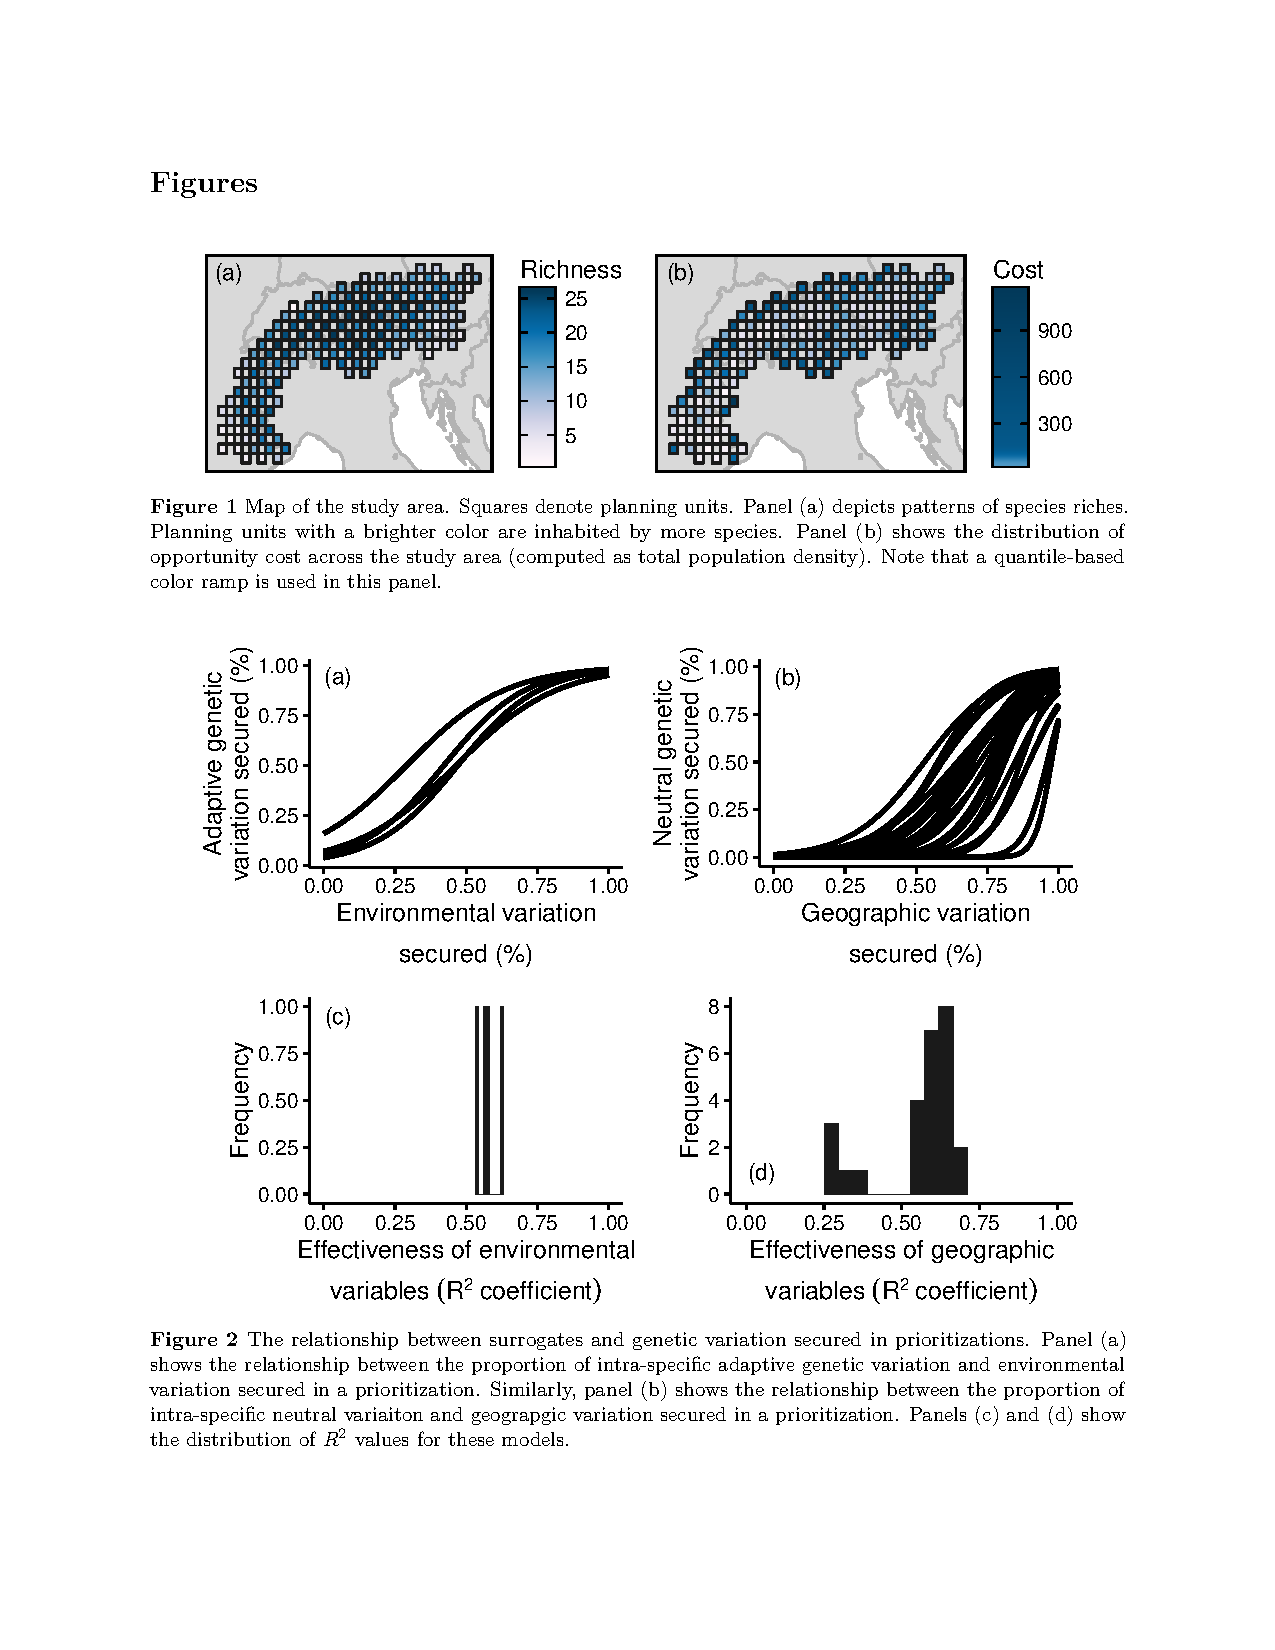
\includepdf[pages=-]{figures.pdf}
\includepdf[pages=-]{supporting_information.pdf}

\end{document}
